\documentclass[11pt,a4paper]{article}
\usepackage[top=16mm,bottom=17mm,left=16mm,right=16mm,headheight=0pt,headsep=0mm,footskip=10mm]{geometry}
\usepackage{iftex}
\ifPDFTeX
  \usepackage[utf8]{inputenc}
  \usepackage[T5]{fontenc}
  \usepackage{mathptmx}
\else
  \usepackage{mathptmx}
  \usepackage{fontspec}
  \IfFontExistsTF{Times New Roman}{\setmainfont{Times New Roman}}{\IfFontExistsTF{TeXGyreTermes}{\setmainfont{TeXGyreTermes}}{\setmainfont{Latin Modern Roman}}}
\fi
\usepackage{amsmath,amssymb}
\usepackage{xcolor,tikz,enumitem,multicol,fancyhdr,lastpage}
\usepackage[most]{tcolorbox}
\definecolor{questionpurple}{RGB}{137,38,143}
\definecolor{answerblue}{RGB}{35,45,140}
\definecolor{lightblue}{RGB}{238,245,255}
\setlength{\parindent}{0pt}
\setlength{\parskip}{0pt}
\renewcommand{\baselinestretch}{1.08}
\setlength{\columnsep}{8mm}
\pagestyle{fancy}
\fancyhf{}
\renewcommand{\headrulewidth}{0pt}
\fancyfoot[L]{\small Chuyên đề III -- Toán 11}
\fancyfoot[R]{\small Trang \thepage/\pageref{LastPage} -- Bài 08.1}
\renewcommand{\footrulewidth}{.4pt}
\setlist[itemize]{leftmargin=6mm,label=\textcolor{answerblue}{\textbullet},itemsep=1pt,topsep=1pt,parsep=0pt}
\setlist[enumerate]{leftmargin=8mm,itemsep=1pt,topsep=1pt,parsep=0pt}
\newtcolorbox{theorybox}{colback=lightblue,colframe=answerblue!60,boxrule=.5pt,
  arc=1mm,left=2.5mm,right=2.5mm,top=1mm,bottom=1mm,before skip=2pt,after skip=2pt}
\newcommand{\sectitle}[2]{\vspace{3pt}\noindent{\large\bfseries\textcolor{questionpurple}{#1.\ #2}}\par\vspace{2pt}}
\newcommand{\exampletitle}[2]{\vspace{2pt}\noindent{\bfseries\textcolor{answerblue}{Ví dụ #1.}} #2\par\vspace{1pt}}
\newcommand{\propertytitle}[1]{\par\vspace{2pt}\noindent\textbf{\textcolor{answerblue}{#1}}\enspace}
\newcommand{\drawpoint}[3]{\fill[answerblue] (#1) circle (1.35pt) node[#2] {$#3$};}
\setlength{\abovedisplayskip}{3pt}
\setlength{\belowdisplayskip}{3pt}
\setlength{\abovedisplayshortskip}{2pt}
\setlength{\belowdisplayshortskip}{2pt}
\raggedbottom

\begin{document}
\noindent
\begin{minipage}[t]{.35\linewidth}
  \centering{\bfseries CHUYÊN ĐỀ III -- TOÁN -- 11\par}
  \vspace{2pt}\rule{.73\linewidth}{.4pt}\par\vspace{2pt}
  CHỦ ĐỀ 03\par\vspace{2pt}{\itshape TÀI LIỆU HỌC TẬP -- BÀI 08.1\par}
\end{minipage}\hfill
\begin{minipage}[t]{.62\linewidth}
  \centering{\bfseries HÌNH HỌC KHÔNG GIAN\par}
  \vspace{4pt}{\small\bfseries VẤN ĐỀ 11X33\par
  ĐƯỜNG THẲNG VÀ MẶT PHẲNG SONG SONG\par}
\end{minipage}

\vspace{3mm}
\noindent\textbf{Họ và tên:}\dotfill\hfill\textbf{Lớp:}\enspace\dotfill
\vspace{1mm}

\begin{theorybox}
\textbf{Kiến thức trọng tâm:} Vị trí tương đối của đường thẳng và mặt phẳng;
dấu hiệu nhận biết đường thẳng song song với mặt phẳng; giao tuyến của
hai mặt phẳng; vận dụng với hình chóp và hình tứ diện.
\end{theorybox}

\sectitle{1}{Đường thẳng song song với mặt phẳng}

Cho đường thẳng $d$ và mặt phẳng $(\alpha)$. Nếu $d$ và $(\alpha)$
\textbf{không có điểm chung}, ta nói $d$ song song với $(\alpha)$,
kí hiệu $d\parallel(\alpha)$ hoặc $(\alpha)\parallel d$.
Trong không gian có ba vị trí tương đối:
\begin{itemize}
  \item $d\parallel(\alpha)$ khi $d\cap(\alpha)=\varnothing$.
  \item $d$ cắt $(\alpha)$ tại duy nhất $M$ khi
  $d\cap(\alpha)=\{M\}$.
  \item $d$ nằm trong $(\alpha)$ khi $d\subset(\alpha)$
  (tương đương $(\alpha)\supset d$).
\end{itemize}
\begin{center}
\begin{minipage}[t]{.32\linewidth}\centering
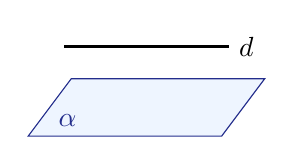
\begin{tikzpicture}[scale=.91]
  \fill[lightblue] (0,0)--(2.7,0)--(3.3,.8)--(.6,.8)--cycle;
  \draw[answerblue] (0,0)--(2.7,0)--(3.3,.8)--(.6,.8)--cycle;
  \draw[thick] (.5,1.25)--(2.8,1.25) node[right] {$d$};
  \node[answerblue] at (.55,.22) {$\alpha$};
\end{tikzpicture}
{\small $d\parallel(\alpha)$}
\end{minipage}\hfill
\begin{minipage}[t]{.32\linewidth}\centering
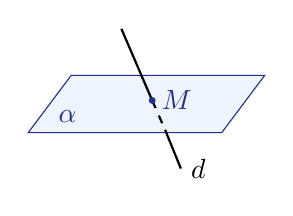
\begin{tikzpicture}[scale=.91]
  \fill[lightblue] (0,0)--(2.7,0)--(3.3,.8)--(.6,.8)--cycle;
  \draw[answerblue] (0,0)--(2.7,0)--(3.3,.8)--(.6,.8)--cycle;
  \draw[thick] (1.3,1.45)--(1.73,.45);
  \draw[thick,dashed] (1.73,.45)--(1.91,.04);
  \draw[thick] (1.91,.04)--(2.13,-.5) node[right] {$d$};
  \drawpoint{1.73,.45}{right}{M}
  \node[answerblue] at (.55,.22) {$\alpha$};
\end{tikzpicture}
{\small $d\cap(\alpha)=\{M\}$}
\end{minipage}\hfill
\begin{minipage}[t]{.32\linewidth}\centering
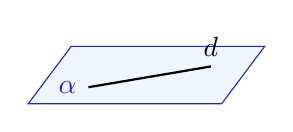
\begin{tikzpicture}[scale=.91]
  \fill[lightblue] (0,0)--(2.7,0)--(3.3,.8)--(.6,.8)--cycle;
  \draw[answerblue] (0,0)--(2.7,0)--(3.3,.8)--(.6,.8)--cycle;
  \draw[thick] (.84,.23)--(2.55,.52) node[above] {$d$};
  \node[answerblue] at (.55,.22) {$\alpha$};
\end{tikzpicture}
{\small $d\subset(\alpha)$}
\end{minipage}
\end{center}

\exampletitle{01 [TDM31]}{Cho tứ diện $ABCD$. Hãy xác định vị trí
tương đối của cạnh $AB$ với bốn mặt phẳng chứa các mặt của tứ diện.}
\begin{center}
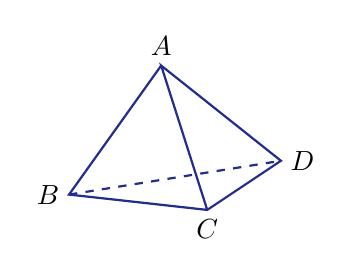
\begin{tikzpicture}[scale=.78]
  \coordinate (A) at (1.5,2.1);
  \coordinate (B) at (0,0);
  \coordinate (C) at (2.25,-.25);
  \coordinate (D) at (3.45,.55);
  \draw[answerblue,thick] (A)--(B)--(C)--(D)--(A)--(C);
  \draw[answerblue,thick,dashed] (B)--(D);
  \node[above] at (A) {$A$}; \node[left] at (B) {$B$};
  \node[below] at (C) {$C$}; \node[right] at (D) {$D$};
\end{tikzpicture}
\end{center}

\sectitle{2}{Điều kiện và tính chất của đường thẳng song song với mặt phẳng}

\propertytitle{Định lí 1.}
Nếu đường thẳng $a$ không nằm trong mặt phẳng $(\alpha)$ và
$a$ song song với đường thẳng $b$ nằm trong $(\alpha)$
thì $a$ song song với $(\alpha)$.
\[
 \boxed{\left.
 \begin{array}{l}
   a\not\subset(\alpha)\\[-1pt]
   a\parallel b\\[-1pt]
   b\subset(\alpha)
 \end{array}\right\}\Longrightarrow a\parallel(\alpha).}
\]
\textbf{Chú ý.} Nếu chỉ biết $a\parallel b$ và $b\subset(\alpha)$,
thì $a\parallel(\alpha)$ \emph{hoặc} $a\subset(\alpha)$.
\begin{center}
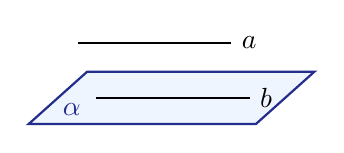
\begin{tikzpicture}[scale=.78]
  \fill[lightblue] (0,0)--(3.7,0)--(4.65,.85)--(.95,.85)--cycle;
  \draw[answerblue,thick] (0,0)--(3.7,0)--(4.65,.85)--(.95,.85)--cycle;
  \draw[thick] (.8,1.32)--(3.3,1.32) node[right] {$a$};
  \draw[thick] (1.1,.42)--(3.6,.42) node[right] {$b$};
  \node[answerblue] at (.7,.24) {$\alpha$};
\end{tikzpicture}
\end{center}

\newpage
\propertytitle{Định lí 2.}
Cho $a\parallel(\alpha)$. Nếu mặt phẳng $(\beta)$ chứa
$a$ và cắt $(\alpha)$ theo giao tuyến $b$ thì $b\parallel a$.
\[
 \boxed{\left.
 \begin{array}{l}
   a\parallel(\alpha)\\[-1pt]
   a\subset(\beta)\\[-1pt]
   (\beta)\cap(\alpha)=b
 \end{array}\right\}\Longrightarrow b\parallel a.}
\]
\begin{center}
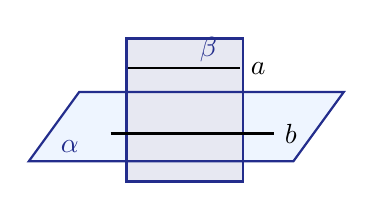
\begin{tikzpicture}[scale=.80]
  \fill[lightblue] (0,0)--(4.2,0)--(5,1.1)--(.8,1.1)--cycle;
  \fill[answerblue!11] (1.55,-.32)--(3.4,-.32)--(3.4,1.95)--(1.55,1.95)--cycle;
  \draw[answerblue,thick] (0,0)--(4.2,0)--(5,1.1)--(.8,1.1)--cycle;
  \draw[answerblue,thick] (1.55,-.32)--(3.4,-.32)--(3.4,1.95)--(1.55,1.95)--cycle;
  \draw[thick] (1.58,1.48)--(3.36,1.48) node[right] {$a$};
  \draw[thick] (1.30,.44)--(3.9,.44) node[right] {$b$};
  \node[answerblue] at (.65,.24) {$\alpha$};
  \node[answerblue] at (2.85,1.78) {$\beta$};
\end{tikzpicture}
\end{center}

\propertytitle{Hệ quả của định lí 2.}
Nếu hai mặt phẳng phân biệt cùng song song với một đường thẳng thì
giao tuyến của chúng (nếu có) cũng song song với đường thẳng đó.
\[
 \boxed{\left.
 \begin{array}{l}
  (\alpha)\ne(\beta)\\[-1pt]
  a\parallel(\alpha),\ a\parallel(\beta)\\[-1pt]
  (\alpha)\cap(\beta)=b
 \end{array}\right\}\Longrightarrow b\parallel a.}
\]

\sectitle{3}{Ví dụ vận dụng}

\exampletitle{01 [TDM31]}{Cho tứ diện $ABCD$. Gọi $M$ là trung điểm của $AC$;
$E,F$ là hai điểm thuộc cạnh $AD$ sao cho $A,E,F,D$ theo thứ tự cách đều nhau.}
\begin{enumerate}
  \item Chứng minh $ME\parallel(BCF)$.
  \item Gọi $(\alpha)$ là mặt phẳng đi qua $M$ và song song với
  $AB,CD$. Tìm giao tuyến của $(\alpha)$ với các mặt của tứ diện $ABCD$.
  Khi nối các giao tuyến này lại, hình thu được là hình gì?
\end{enumerate}
\begin{center}
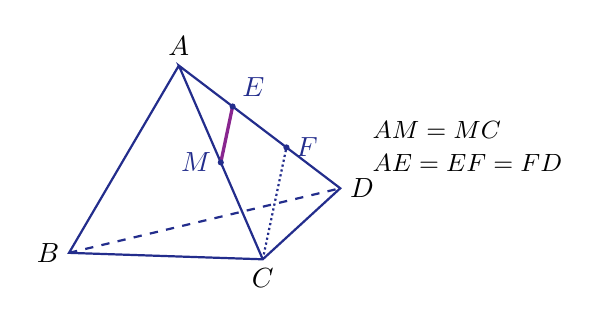
\begin{tikzpicture}[scale=.82]
  \coordinate (A) at (1.7,2.9);
  \coordinate (B) at (0,0);
  \coordinate (C) at (3,-.1);
  \coordinate (D) at (4.2,1);
  \coordinate (M) at (2.35,1.4);
  \coordinate (E) at (2.533,2.267);
  \coordinate (F) at (3.367,1.633);
  \draw[answerblue,thick] (A)--(B)--(C)--(D)--(A)--(C);
  \draw[answerblue,thick,dashed] (B)--(D);
  \draw[answerblue,thick,densely dotted] (C)--(F);
  \draw[questionpurple,very thick] (M)--(E);
  \node[above] at (A) {$A$}; \node[left] at (B) {$B$};
  \node[below] at (C) {$C$}; \node[right] at (D) {$D$};
  \drawpoint{2.35,1.4}{left}{M}
  \drawpoint{2.533,2.267}{above right}{E}
  \drawpoint{3.367,1.633}{right}{F}
  \node[align=left,right] at (4.55,1.65)
    {\small $AM=MC$\\[-1pt]\small $AE=EF=FD$};
\end{tikzpicture}
\end{center}

\exampletitle{02 [TDM32]}{Trong không gian, cho hai đường thẳng
$a,b$ chéo nhau. Chứng minh rằng có đúng một mặt phẳng chứa
đường thẳng $a$ và song song với đường thẳng $b$.}

\begin{tcolorbox}[colback=white,colframe=black!35,boxrule=.4pt,arc=0mm,
 left=2mm,right=2mm,top=1mm,bottom=1mm,before skip=3pt]
\footnotesize
\textbf{Nguồn nội dung:} TƯ DUY MỞ, \emph{Vấn đề 11X33:
Đường thẳng và mặt phẳng song song}, biên soạn Nguyễn Đăng Ái, trang 1--3
(PDF được cung cấp). Đã biên tập lại thành LaTeX, vẽ lại hình minh họa;
lược bỏ các ô trống làm bài, quảng cáo và nền giấy kẻ.
Tài liệu gốc không cung cấp lời giải cho các ví dụ.
\end{tcolorbox}
\end{document}
